% flashcards-title: Powers-of-ten scale ladder from one millimeter to one kilometer
% flashcards-desc: A vertical ladder of evenly spaced rungs labeled from one millimeter at the bottom through one kilometer at the top, with a note that each step upward multiplies by ten. A circled marker sits at the one-centimeter rung labeled fingernail width, and a squared marker sits at the hundred-meter rung labeled city block.
\documentclass[dvisvgm,tikz,border=8pt]{standalone}
\usepackage{tikz}
\usetikzlibrary{arrows.meta,calc,positioning}
\definecolor{DeckInk}{HTML}{172A3A}
\definecolor{DeckAccent}{HTML}{176B87}
\definecolor{DeckWarm}{HTML}{D97706}
\definecolor{DeckMuted}{HTML}{667784}
\definecolor{DeckPaper}{HTML}{F7FAFC}
\tikzset{
  every node/.style={font=\sffamily, text=DeckInk},
  object/.style={draw=DeckInk, line width=1.1pt, fill=DeckPaper},
  primary/.style={draw=DeckAccent, line width=1.5pt},
  boundary/.style={draw=DeckAccent, line width=1.5pt, dashed, rounded corners=6pt},
  guide/.style={draw=DeckMuted, line width=0.9pt, dashed},
  dimension/.style={{Stealth[length=3.2mm,width=2.2mm]}-{Stealth[length=3.2mm,width=2.2mm]}, draw=DeckWarm, line width=1.2pt},
  motion/.style={-{Stealth[length=3.5mm,width=2.5mm]}, draw=DeckAccent, line width=1.5pt, dashed},
}

\begin{document}
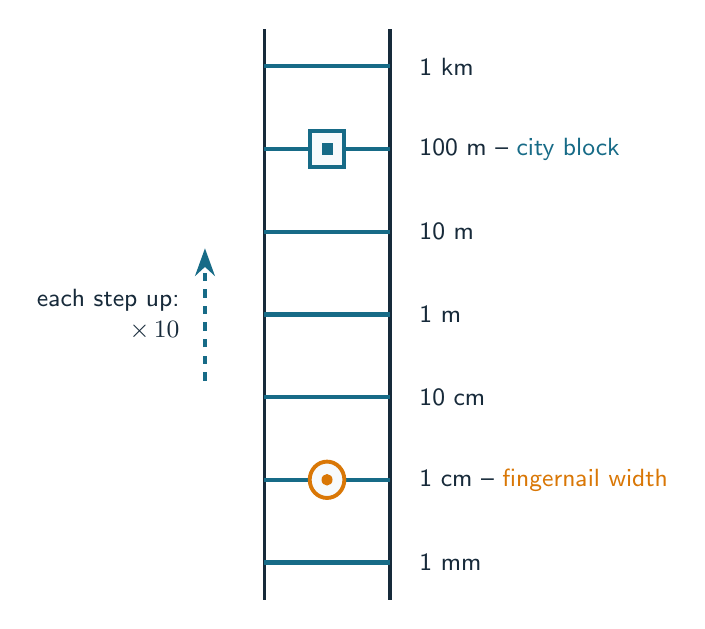
\begin{tikzpicture}[y=1.05cm]
  % Rails
  \draw[object] (0,-0.45) -- (0,6.45);
  \draw[object] (1.6,-0.45) -- (1.6,6.45);
  % Rungs and labels
  \foreach \y/\lbl in {0/1 mm, 2/10 cm, 3/1 m, 4/10 m, 6/1 km} {
    \draw[primary] (0,\y) -- (1.6,\y);
    \node[right, font=\sffamily\small] at (1.85,\y) {\lbl};
  }
  % Marked rungs with combined labels
  \draw[primary] (0,1) -- (1.6,1);
  \node[right, font=\sffamily\small] at (1.85,1)
    {1 cm -- \textcolor{DeckWarm}{fingernail width}};
  \draw[primary] (0,5) -- (1.6,5);
  \node[right, font=\sffamily\small] at (1.85,5)
    {100 m -- \textcolor{DeckAccent}{city block}};
  % Step note with upward arrow on the left
  \draw[motion] (-0.75,2.2) -- (-0.75,3.8);
  \node[left, font=\sffamily\small, align=right] at (-0.95,3.0)
    {each step up:\\ $\times\,10$};
  % Circled marker: fingernail width at 1 cm
  \draw[DeckWarm, line width=1.4pt, fill=DeckPaper] (0.8,1) circle (0.22);
  \fill[DeckWarm] (0.8,1) circle (0.07);
  % Squared marker: city block at 100 m
  \draw[DeckAccent, line width=1.4pt, fill=DeckPaper] (0.58,4.78) rectangle (1.02,5.22);
  \fill[DeckAccent] (0.73,4.93) rectangle (0.87,5.07);
\end{tikzpicture}
\end{document}
